\documentclass[10pt,twocolumn]{article}
\usepackage{xcolor}
\usepackage{comment}
\usepackage{graphicx}
\usepackage{multicol,graphicx}
\usepackage{multirow}
\usepackage{multicol}
\usepackage{subcaption}
\usepackage{tikz}
\usepackage{hyperref}
\usepackage[export]{adjustbox}
\usepackage{circuitikz}
\usepackage{siunitx} %to allign according to decimal point
\usepackage{algorithm2e}
\usepackage{amsmath}
\usepackage{systeme}
\usepackage{lipsum}
\usepackage{blindtext}

\begin{document}
	\title{Preparing Document in LaTex}
	\author{Priyanshu Singh}
	\date{\today}
	\maketitle
	\blindtext
	\begin{figure*}[h]
		\begin{subfigure}[c]{0.45\textwidth}
			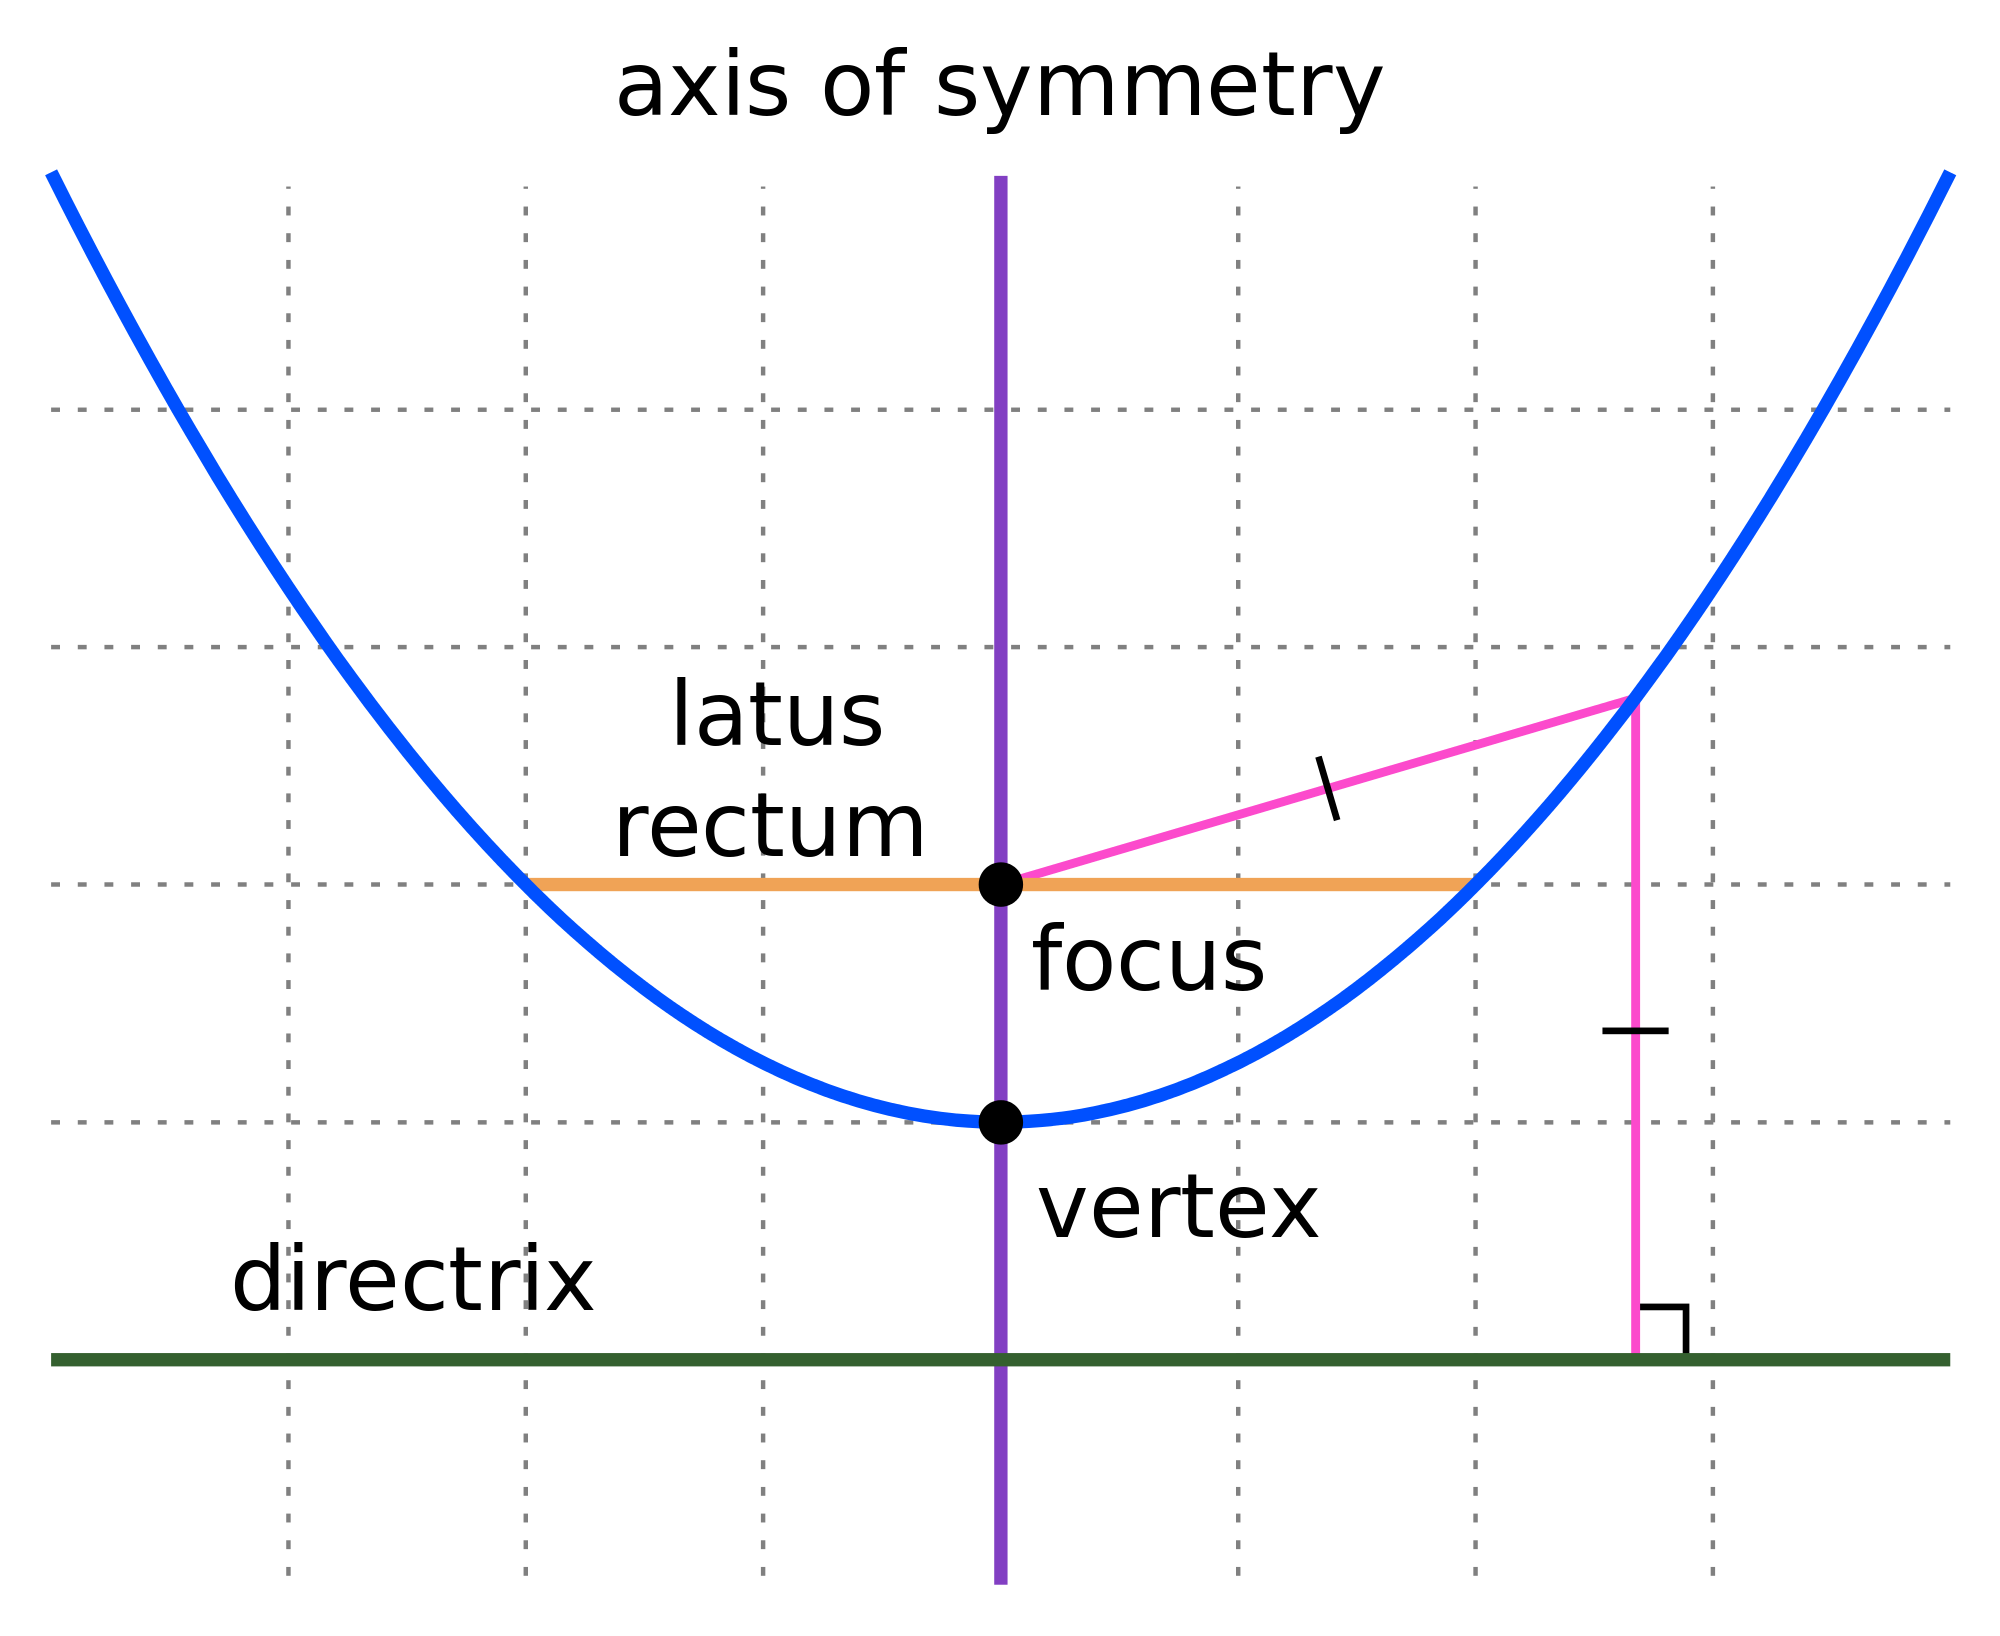
\includegraphics[width=.75\textwidth,right]{parabola}
			\centering
			\label{1a}
			\begin{flushright}\caption{Parabola 1}\end{flushright}
		\end{subfigure}
		\hfill
		\begin{subfigure}[c]{0.45\textwidth}
			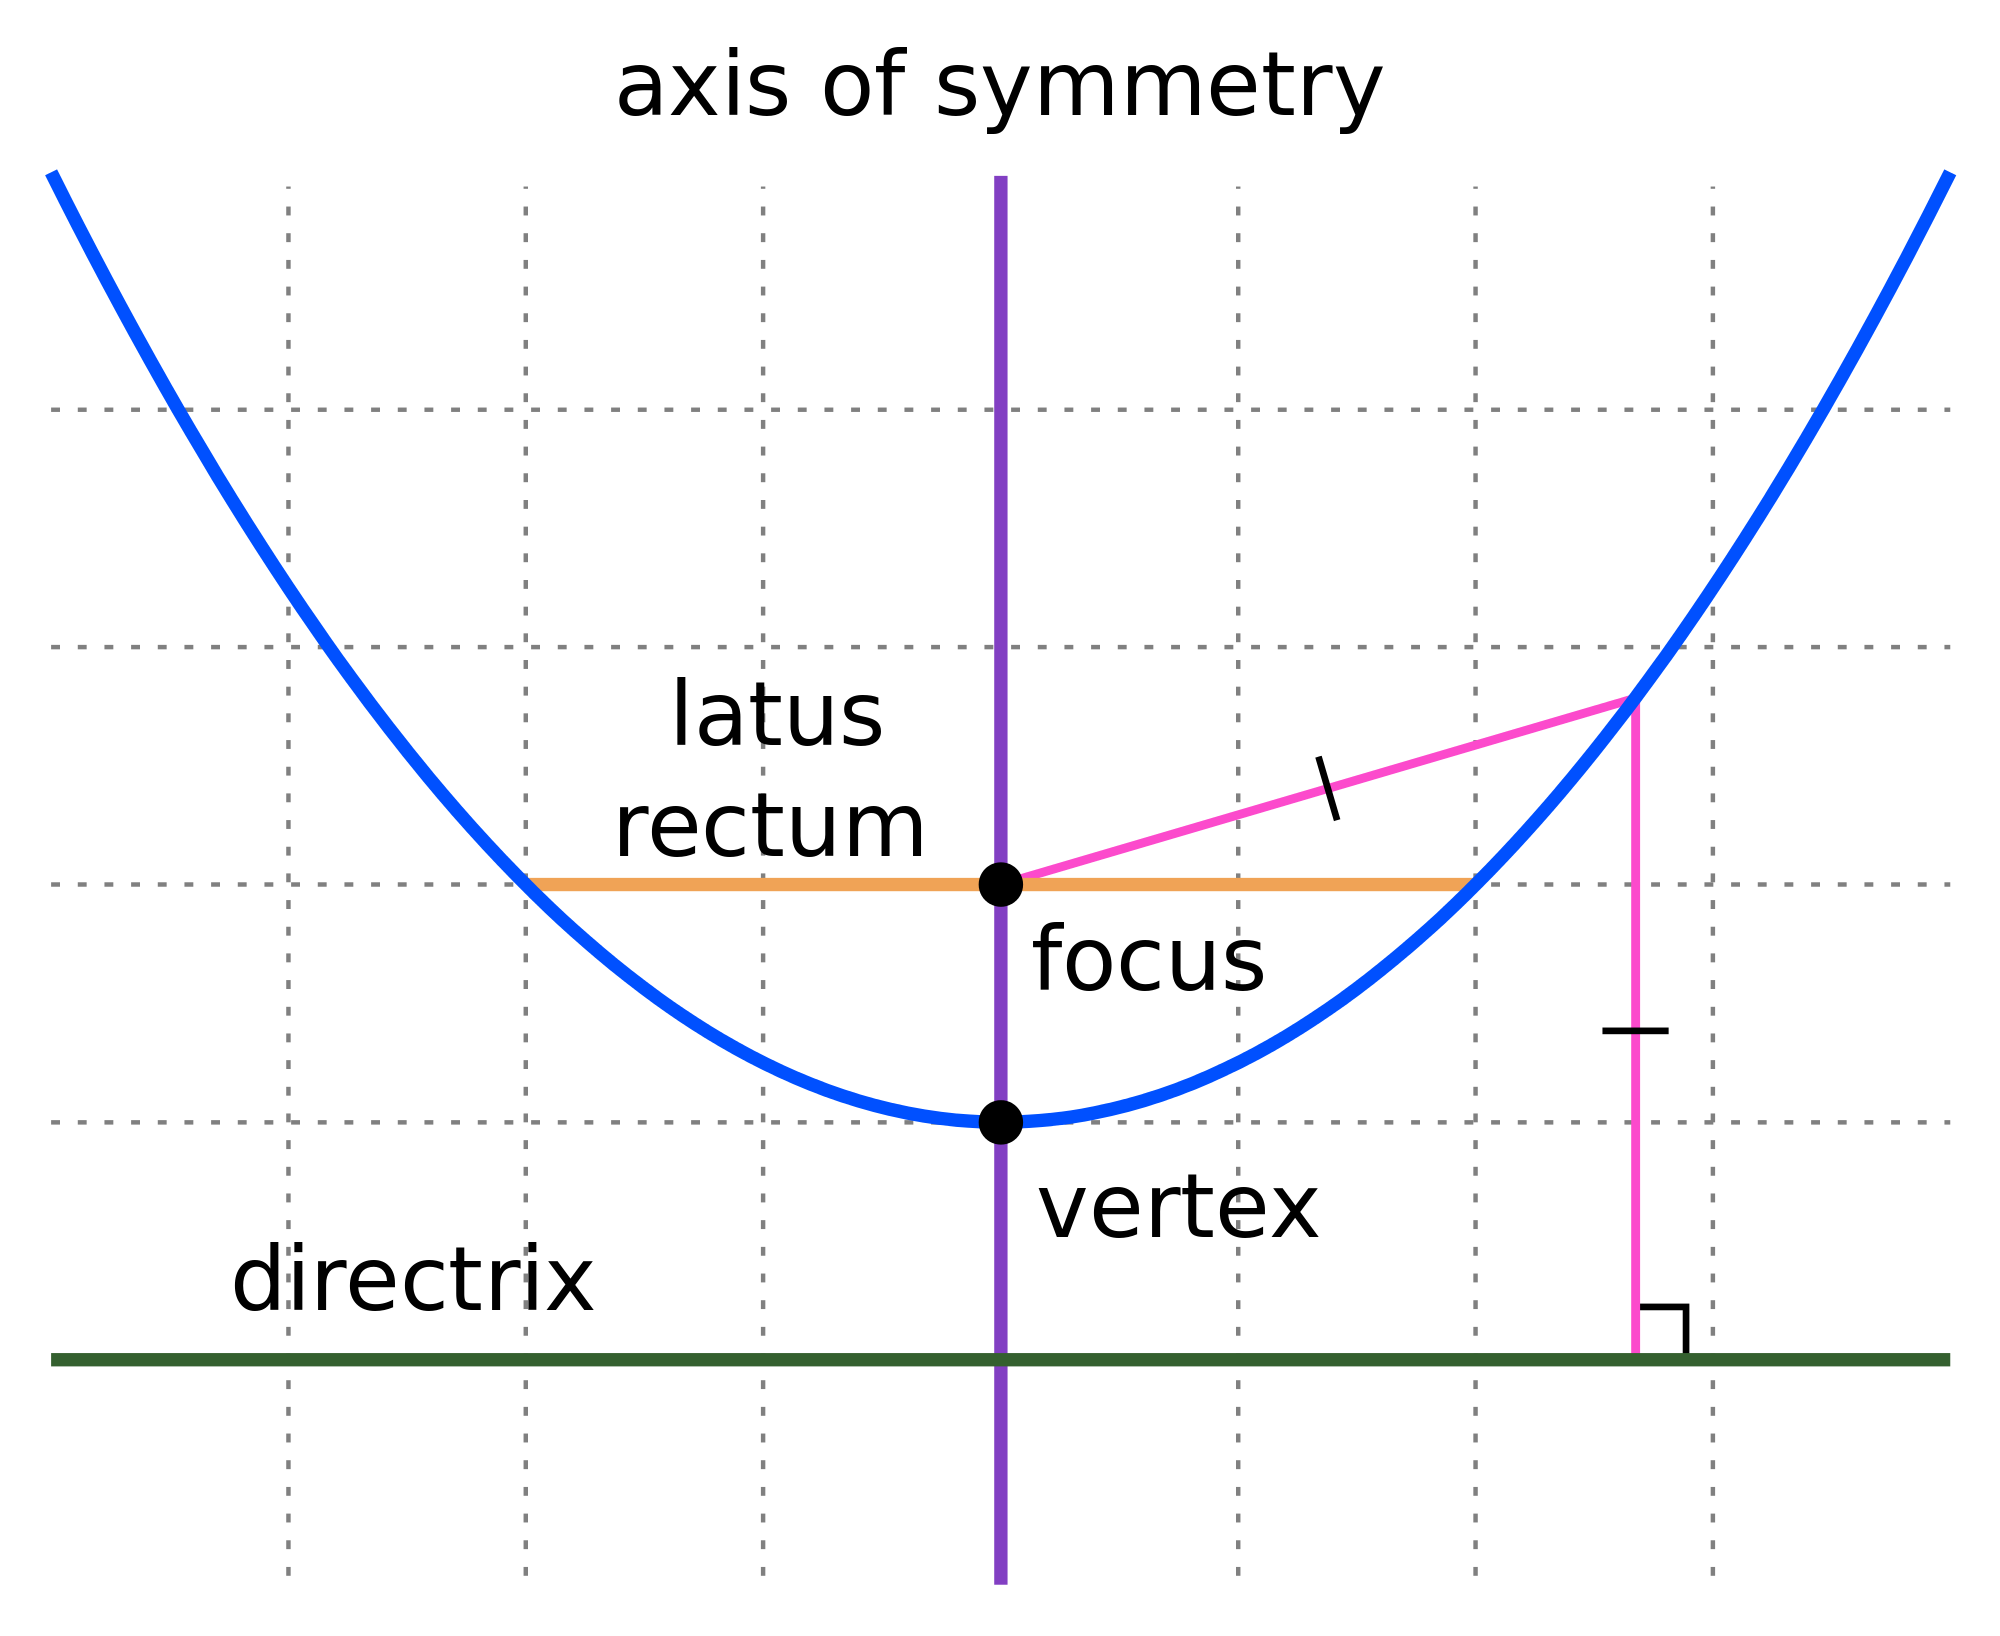
\includegraphics[width=.75\textwidth,left]{parabola}
			\centering
			\begin{center}\caption{Parabola 2}\end{center}
		\end{subfigure}\\
	\end{figure*}
	\blindtext
	\lipsum
	\textcolor{red}{Figure \ref{1a} is referrred here}
\end{document}